\documentclass[11pt,a4paper]{article}
\usepackage[T1]{fontenc}
\usepackage[utf8]{inputenc}
\usepackage[french]{babel}
\usepackage{lmodern}
\usepackage{geometry}
\usepackage{graphicx}
\usepackage{caption}
\usepackage{enumitem}
\usepackage{hyperref}

\geometry{margin=1.7cm}
\setlength{\parskip}{0.6em}
\setlist{nosep,leftmargin=*}
\graphicspath{{screenshots/}}

\title{\vspace{-1.4cm}\textbf{Expense Tracker}\\\large Rapport de projet --- ENSIIE FISA Bases du Web}
\author{Algassimou Pellel DIALLO}
\date{Novembre 2026}

\begin{document}
\maketitle
\thispagestyle{empty}

\section*{1. Technologies utilisées}
Expense Tracker est une application web de suivi de dépenses personnelles. Le serveur est développé avec \textbf{Python 3} et le framework \textbf{Flask}. Ce choix répond aux contraintes du projet : Flask est léger pour une machine virtuelle limitée à 500 Mo de mémoire et produit une archive finale inférieure à 3 Mo. Il correspond aussi à mon expérience préalable avec ce framework. Les données sont enregistrées dans une base \textbf{SQLite} composée de trois tables : \texttt{users}, \texttt{categories} et \texttt{expenses}. L'interface est réalisée en \textbf{HTML}, \textbf{CSS} et \textbf{JavaScript}, sans dépendance externe côté client.

Le code serveur sépare la configuration de l'application, l'authentification, l'accès à la base de données et la gestion des dépenses. La base est créée à partir de \texttt{src/schema.sql}. Le fichier \texttt{README.md} explique l'installation des dépendances et le démarrage du serveur de développement.

\section*{2. Utilisation du site}
L'utilisateur commence par créer un compte avec un pseudo, un email, un mot de passe et un budget mensuel facultatif. Après la connexion, une session signée est ouverte pour une durée de quinze minutes d'inactivité. Les pages privées restent ainsi protégées et l'utilisateur peut se déconnecter à tout moment.

Le tableau de bord présente le budget mensuel, le montant dépensé, le reste disponible, les dépenses récentes et la répartition des dépenses par catégorie. Le bouton \og Ajouter une dépense \fg{} dirige directement vers le formulaire de saisie. Dans la page \og Mes dépenses \fg{}, il est possible d'ajouter, modifier ou supprimer une dépense, puis de la rechercher par nom, catégorie ou mois. Les résultats sont filtrés sans rechargement de page et affichés par groupes de dix. Un histogramme permet de consulter l'évolution des dépenses mensuelles.

Le bouton FR/EN traduit l'interface et conserve la langue choisie lors de la navigation. Le bouton Mobile/Bureau permet de vérifier les deux mises en page. Enfin, la page Contact regroupe les crédits du projet et l'adresse de contact.

\section*{3. Détails techniques}
Après une connexion réussie, Flask stocke uniquement l'identifiant de l'utilisateur dans une session signée. Toutes les routes privées utilisent le décorateur \texttt{login\_required}. Les requêtes de lecture, de modification et de suppression sont systématiquement limitées à cet identifiant : un utilisateur ne peut donc pas consulter ou modifier les dépenses d'un autre compte. Les mots de passe sont conservés sous forme de hachage avec Werkzeug.

La traduction repose sur les attributs \texttt{data-fr} et \texttt{data-en} présents dans les éléments de l'interface. JavaScript remplace le texte affiché et mémorise le choix dans le navigateur. Le même script gère les filtres, la pagination et les notifications de validation. Une page 404 personnalisée est affichée lorsqu'une adresse demandée n'existe pas.

\clearpage
\section*{Captures d'écran}
Les captures suivantes présentent les cinq pages principales dans les deux langues et les deux mises en page demandées. Chaque bloc contient, dans l'ordre, les versions française bureau, anglaise bureau, française mobile et anglaise mobile.

\subsection*{Connexion}
\begin{center}
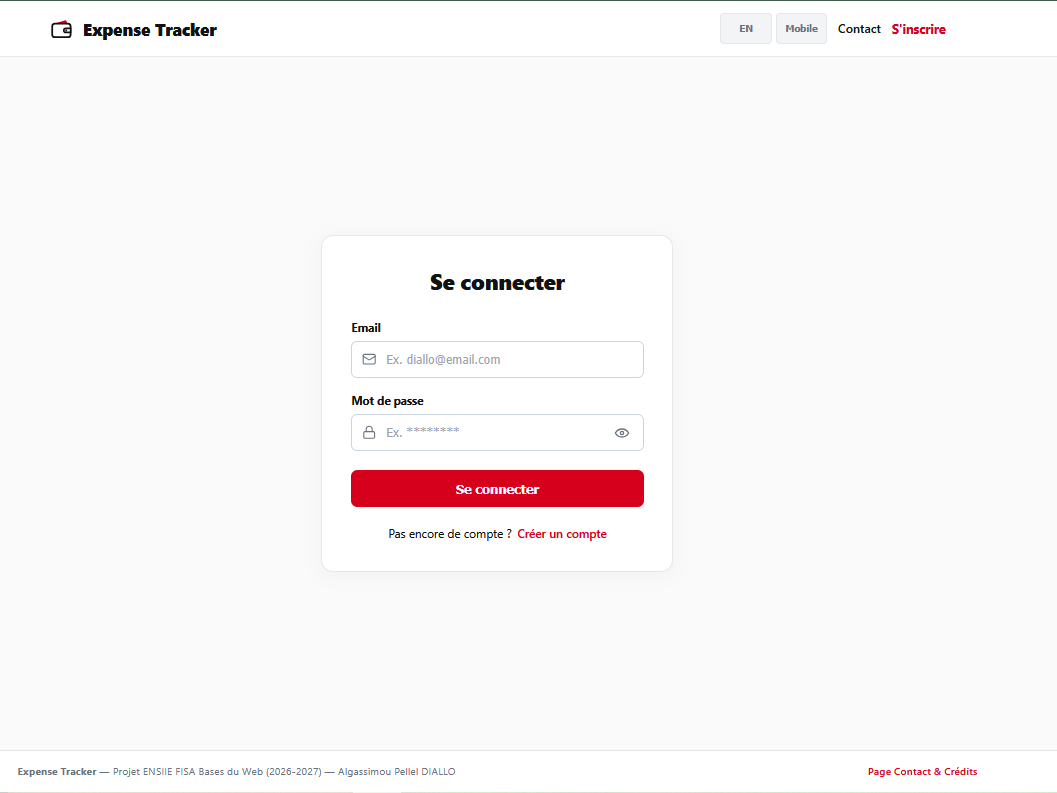
\includegraphics[width=.49\linewidth,height=.29\textheight,keepaspectratio]{login_fr_laptop.png}
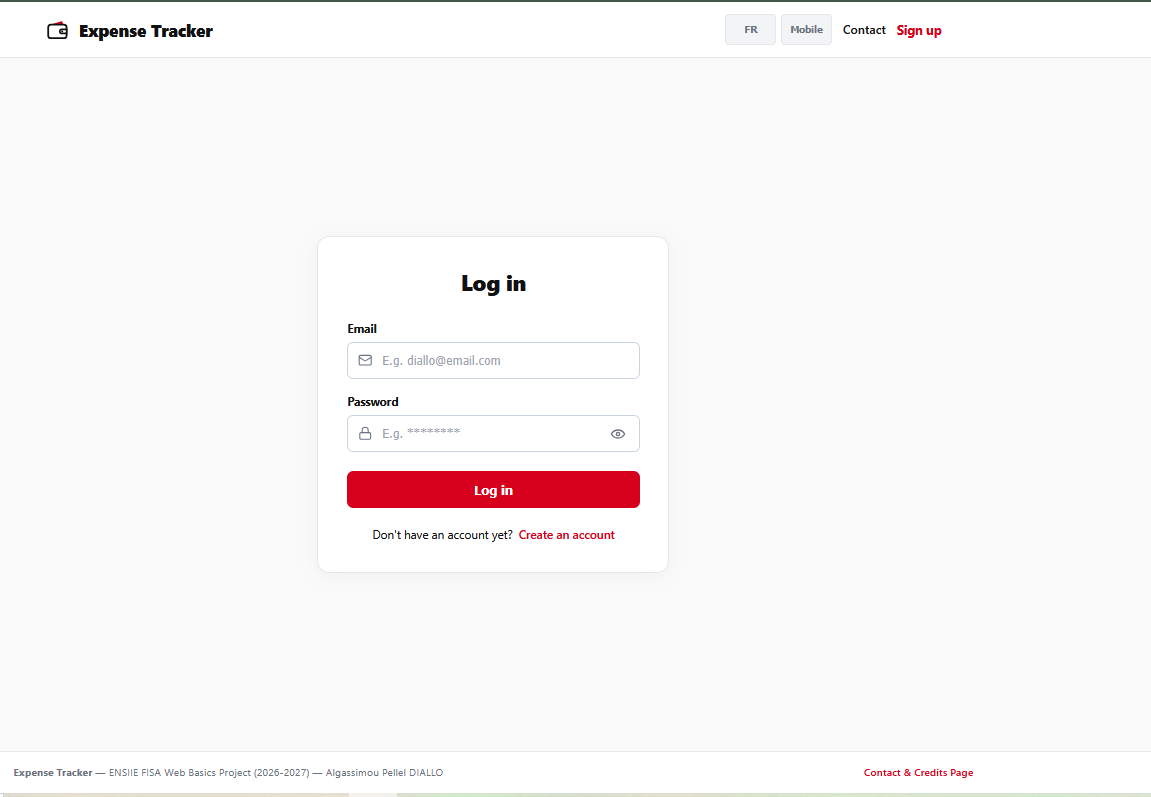
\includegraphics[width=.49\linewidth,height=.29\textheight,keepaspectratio]{login_en_laptop.png}\\
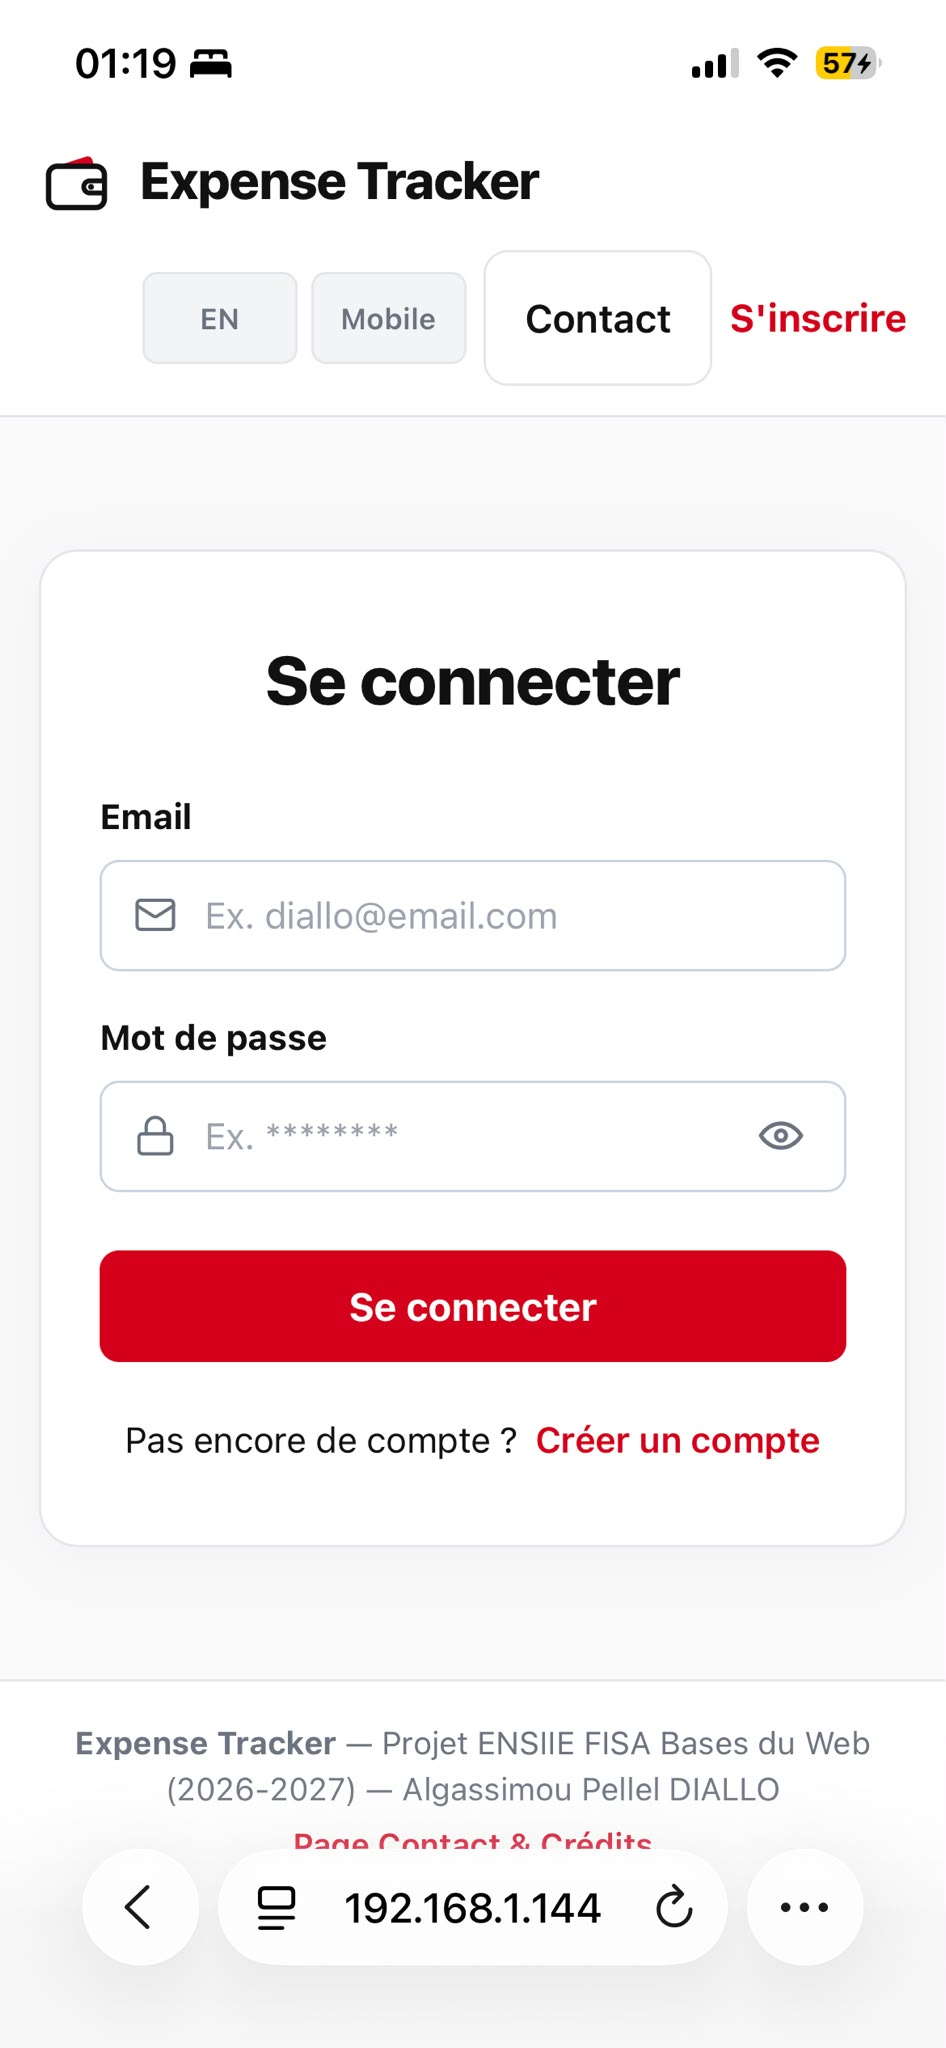
\includegraphics[width=.49\linewidth,height=.29\textheight,keepaspectratio]{login_fr_m.jpeg}
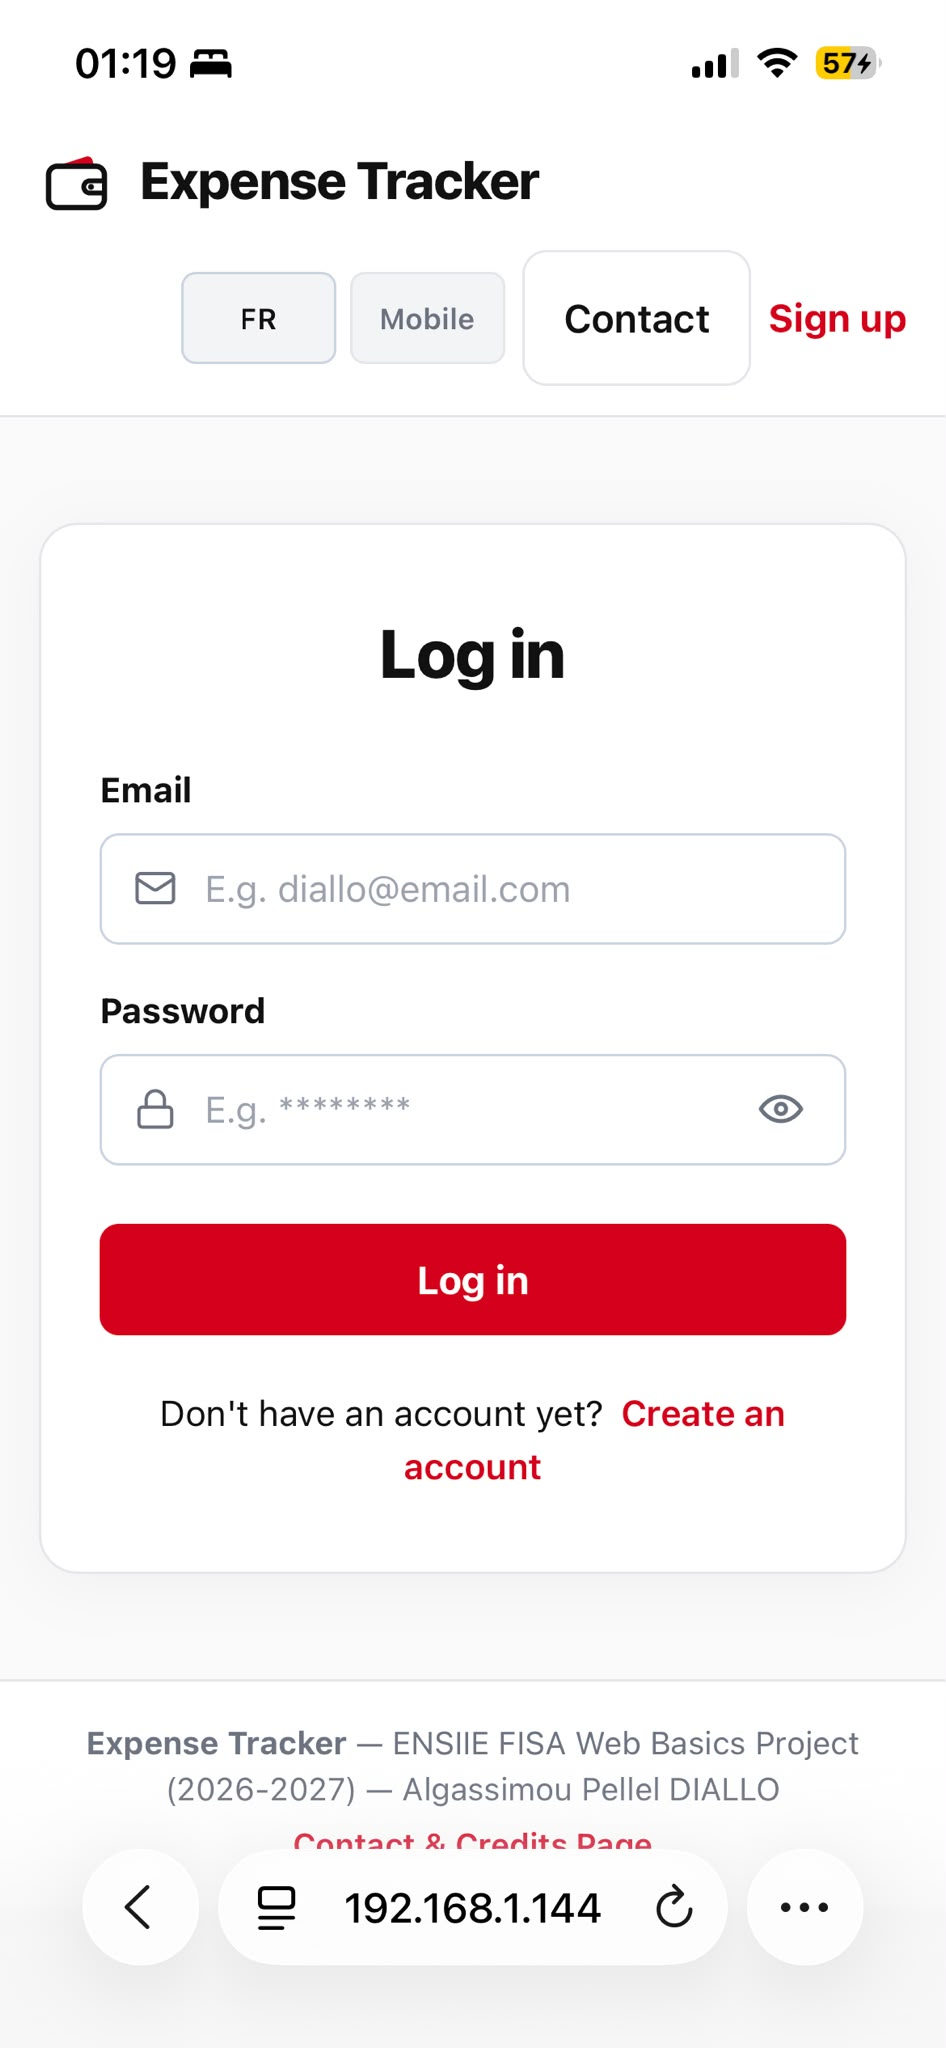
\includegraphics[width=.49\linewidth,height=.29\textheight,keepaspectratio]{login_en_m.jpeg}
\end{center}

\subsection*{Création de compte}
\begin{center}
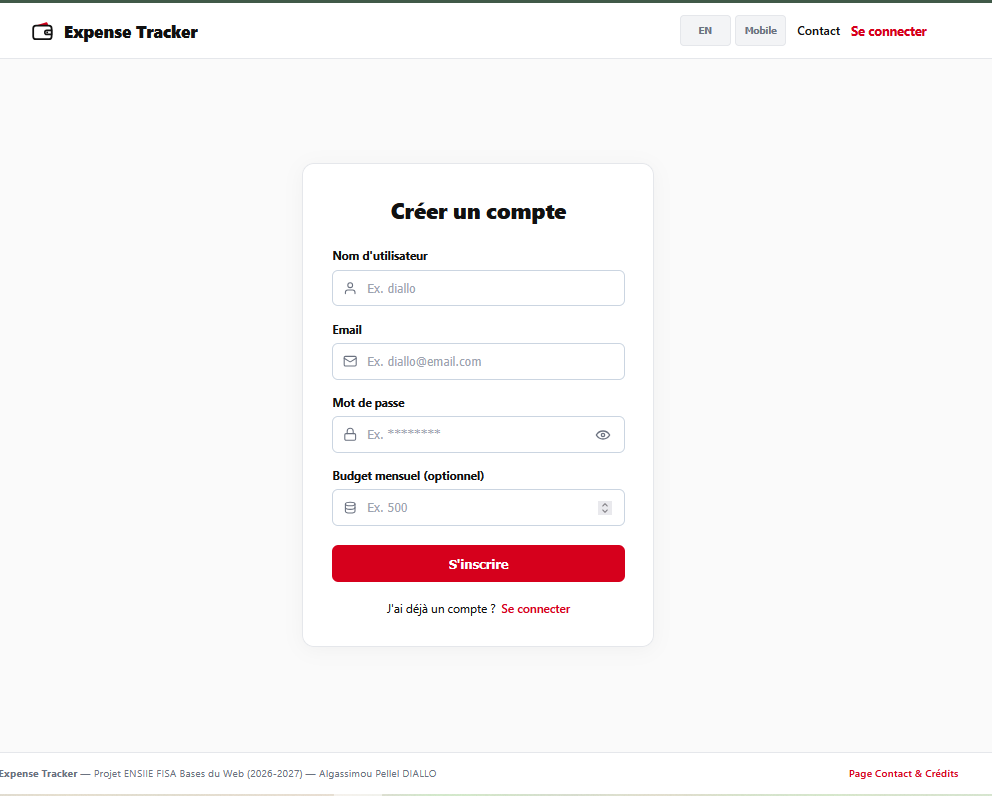
\includegraphics[width=.49\linewidth,height=.29\textheight,keepaspectratio]{creer_compte_fr_laptop.png}
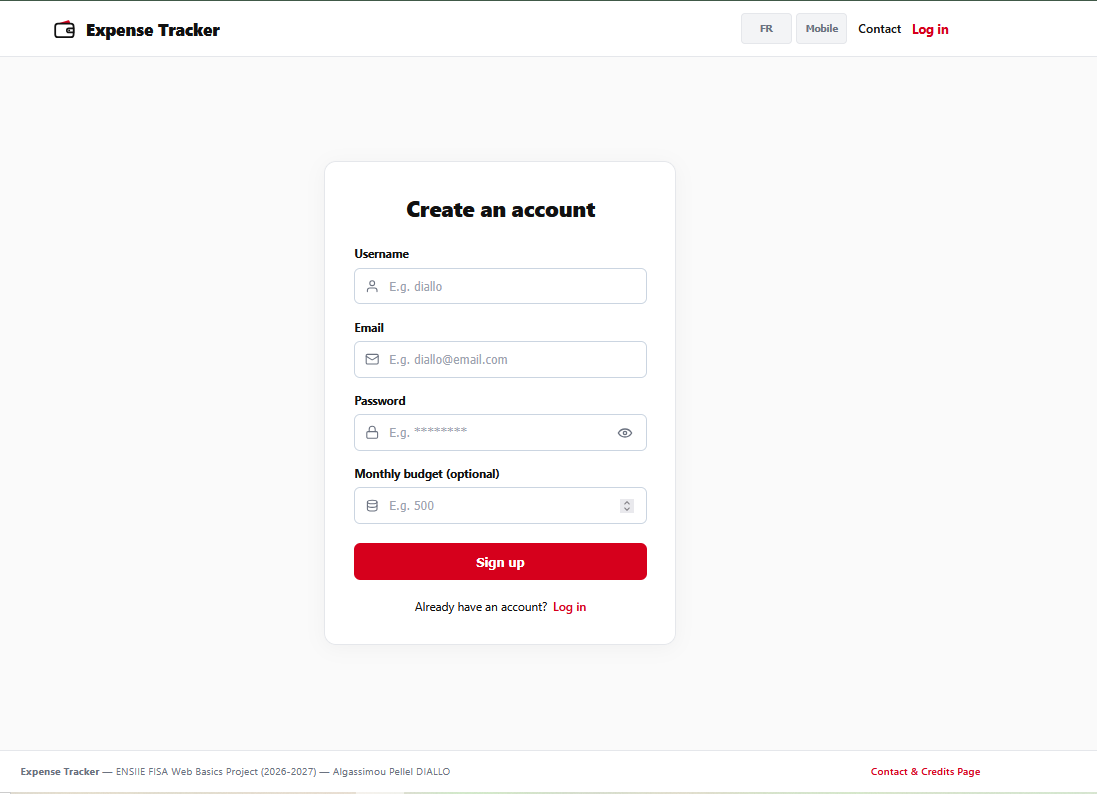
\includegraphics[width=.49\linewidth,height=.29\textheight,keepaspectratio]{creer_compte_en_laptop.png}\\
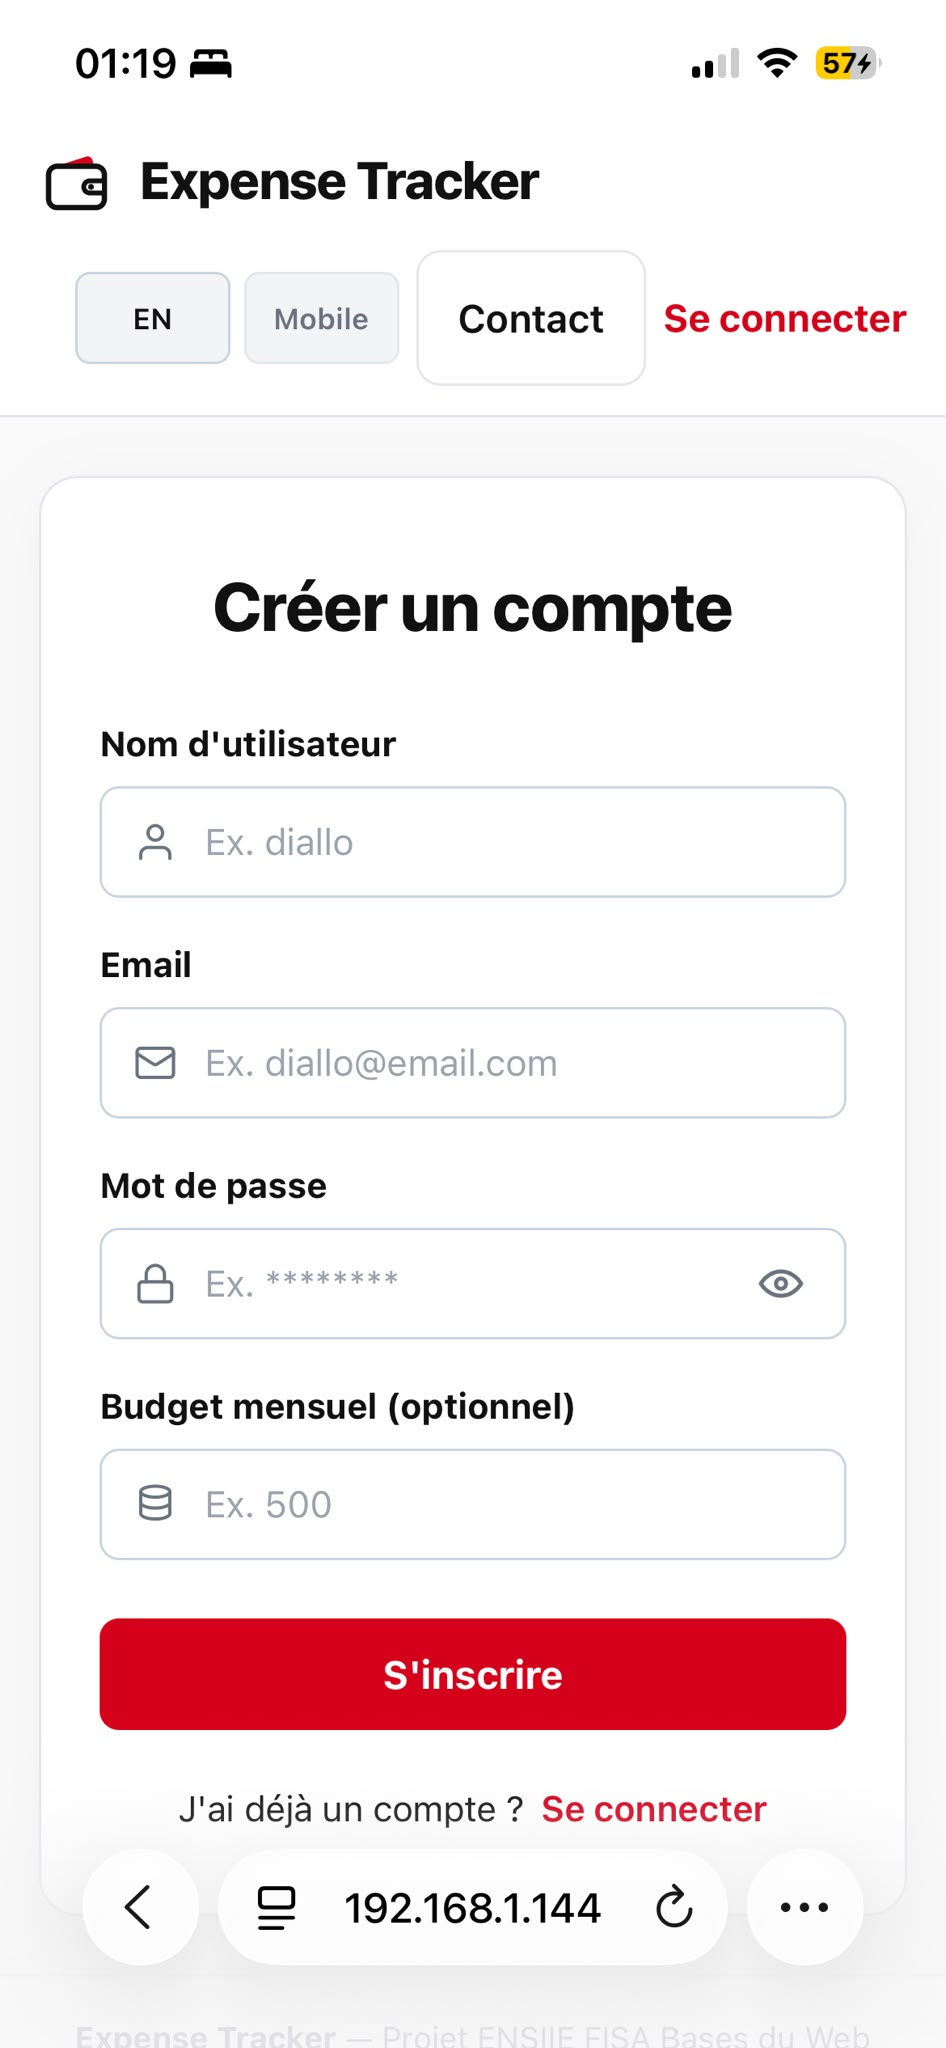
\includegraphics[width=.49\linewidth,height=.29\textheight,keepaspectratio]{creer_compte_fr_m.jpeg}
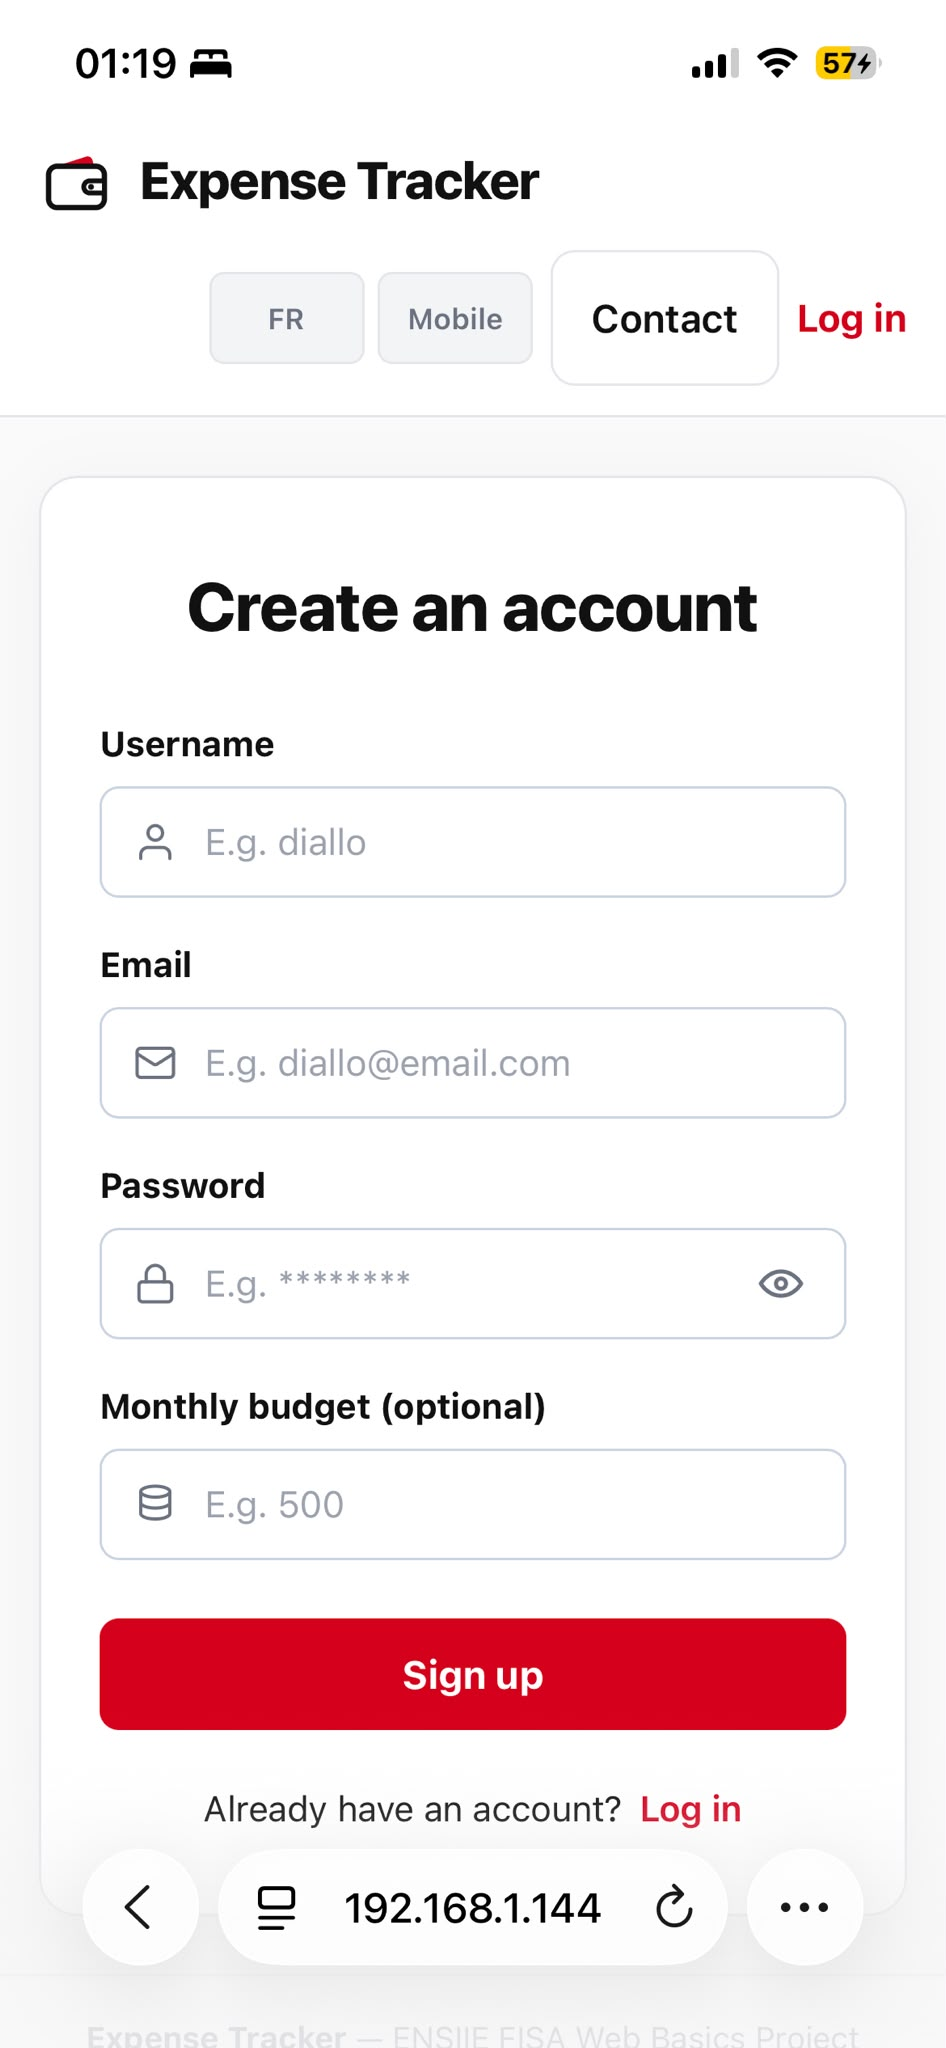
\includegraphics[width=.49\linewidth,height=.29\textheight,keepaspectratio]{creer_cpmpte_en_m.jpeg}
\end{center}

\subsection*{Tableau de bord}
\begin{center}
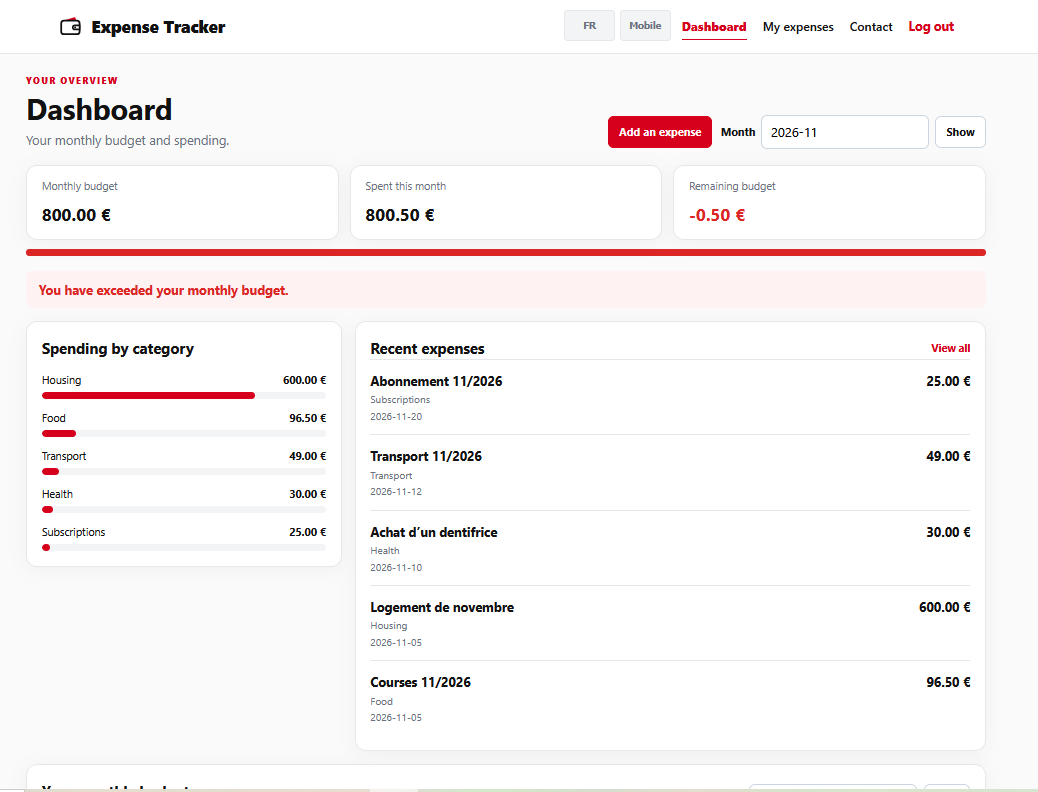
\includegraphics[width=.49\linewidth,height=.29\textheight,keepaspectratio]{dash_fr_laptop.png}
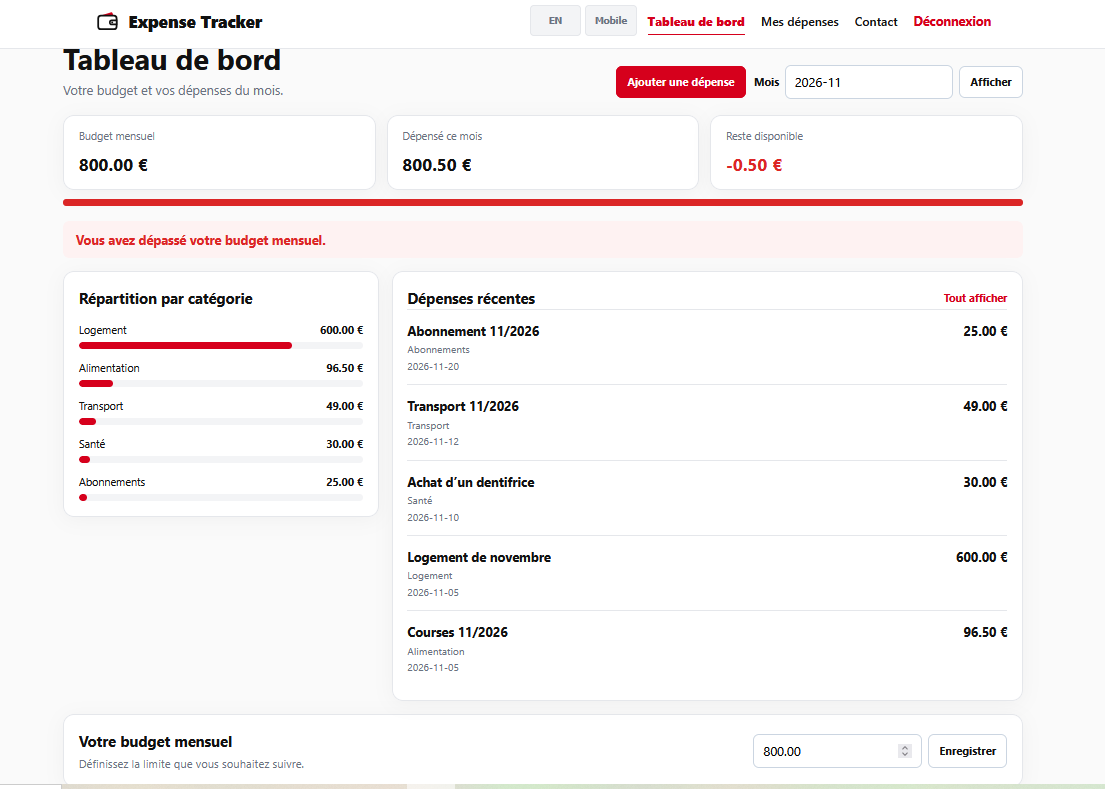
\includegraphics[width=.49\linewidth,height=.29\textheight,keepaspectratio]{dash_en_laptop.png}\\
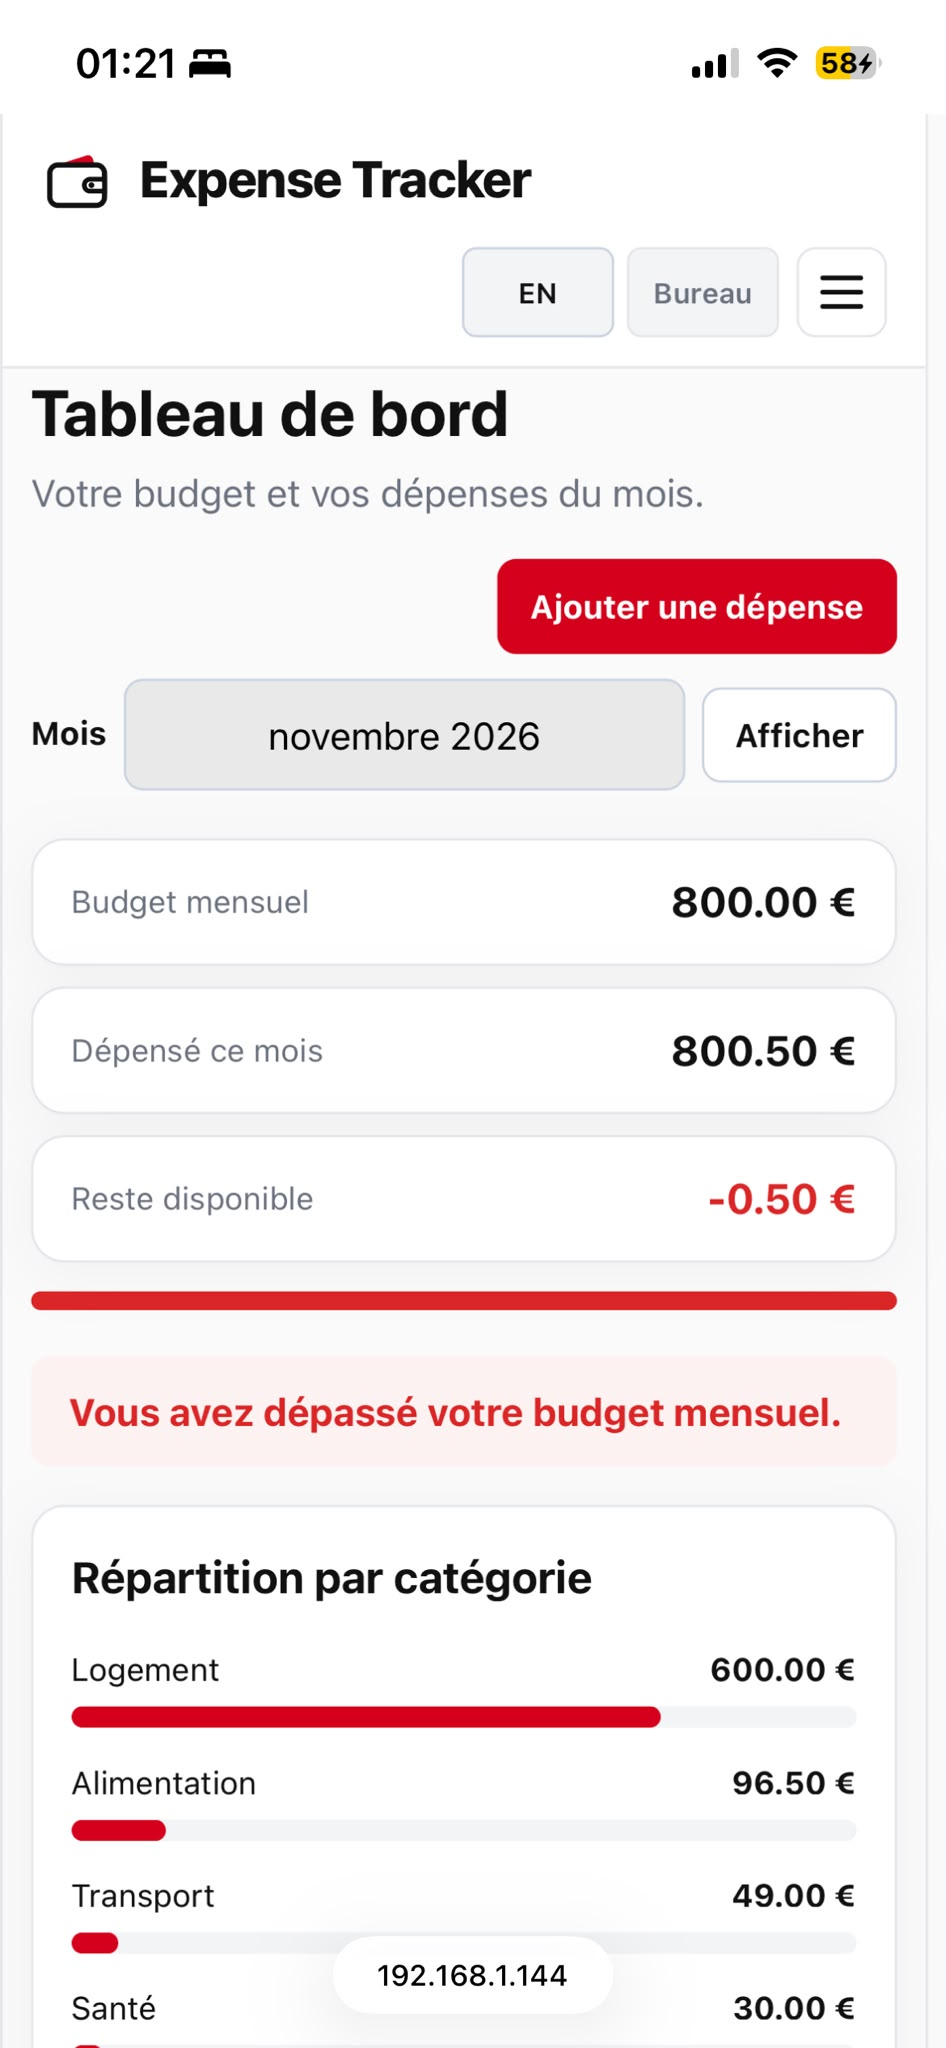
\includegraphics[width=.49\linewidth,height=.29\textheight,keepaspectratio]{tableau_de_bord_fr_m.jpeg}
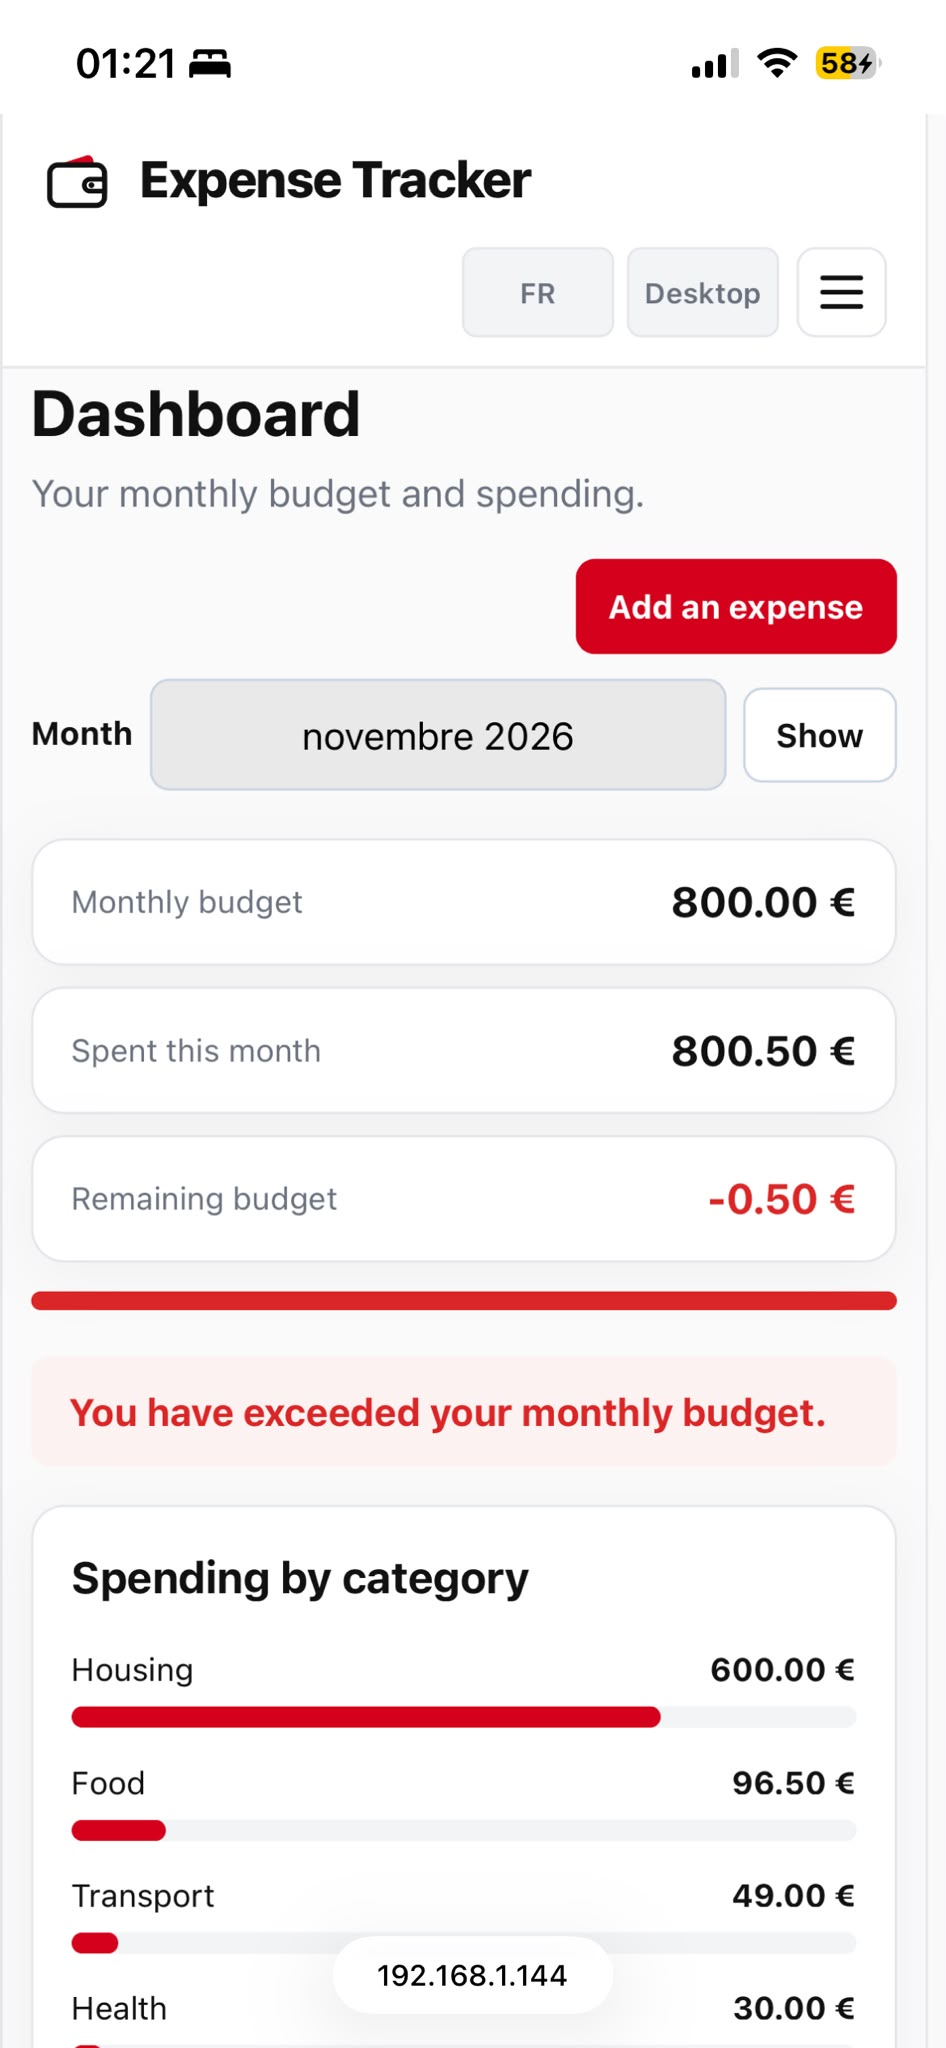
\includegraphics[width=.49\linewidth,height=.29\textheight,keepaspectratio]{tableau_de_bord_en_m.jpeg}
\end{center}

\subsection*{Mes dépenses}
\begin{center}
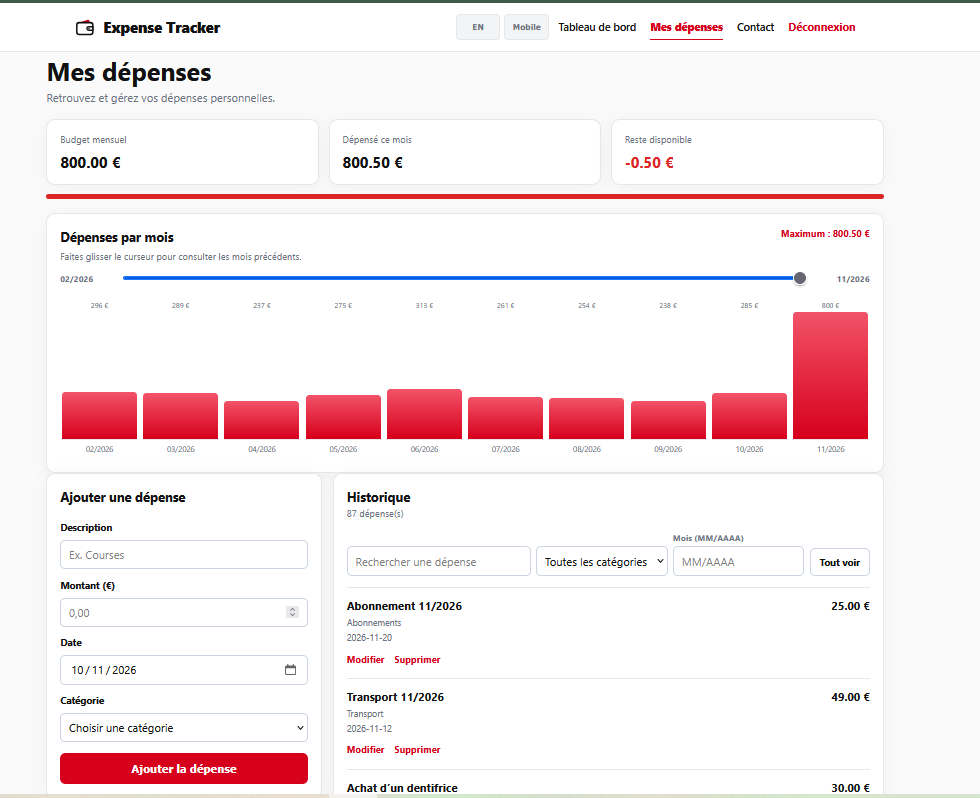
\includegraphics[width=.49\linewidth,height=.29\textheight,keepaspectratio]{expense_fr_laptop.png}
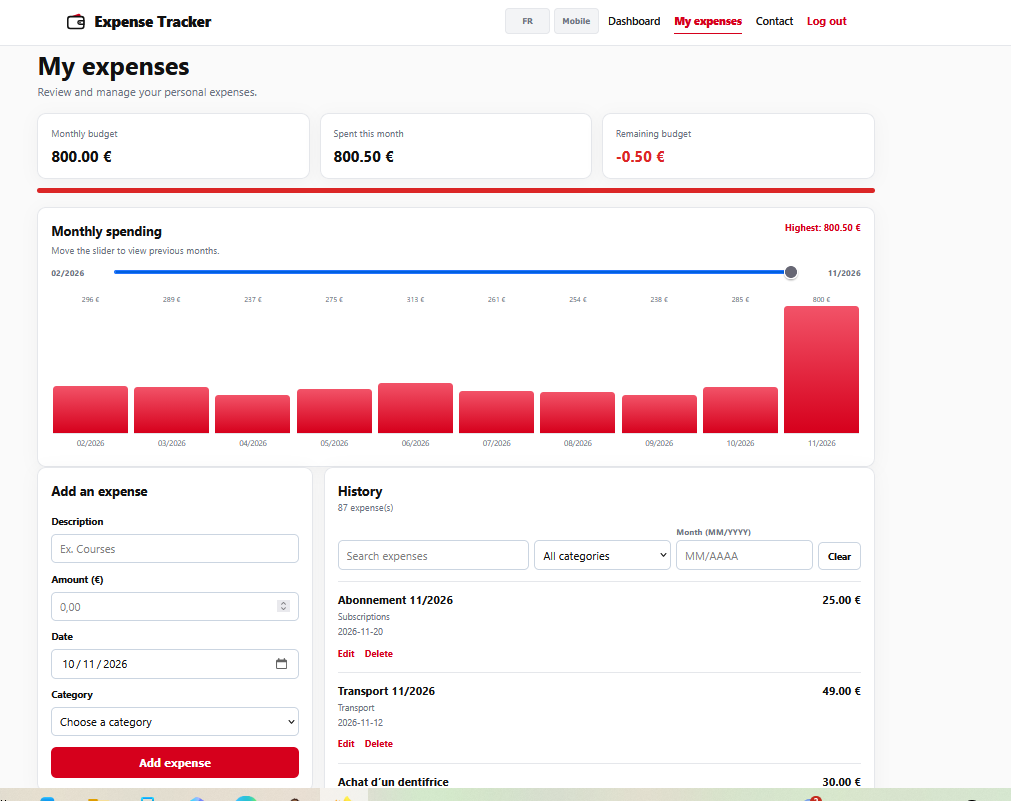
\includegraphics[width=.49\linewidth,height=.29\textheight,keepaspectratio]{expense_en_laptop.png}\\
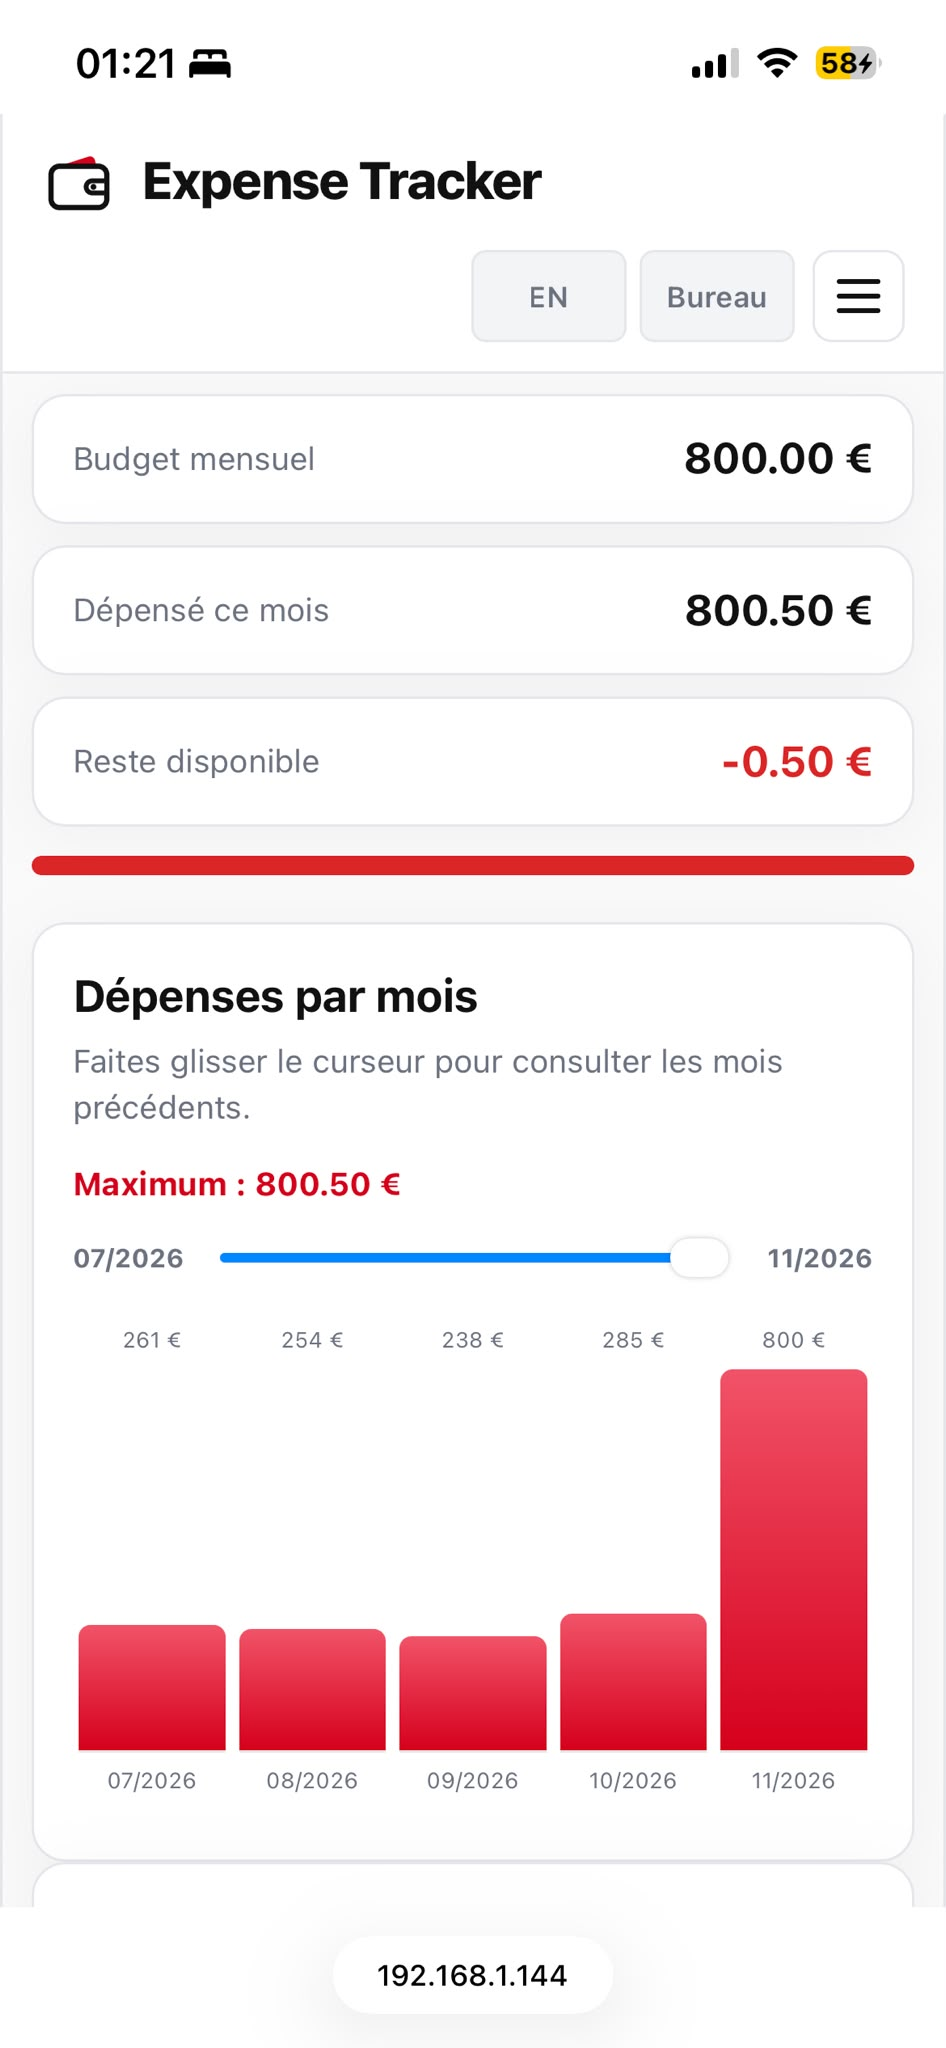
\includegraphics[width=.49\linewidth,height=.29\textheight,keepaspectratio]{my_expense_fr_m.jpeg}
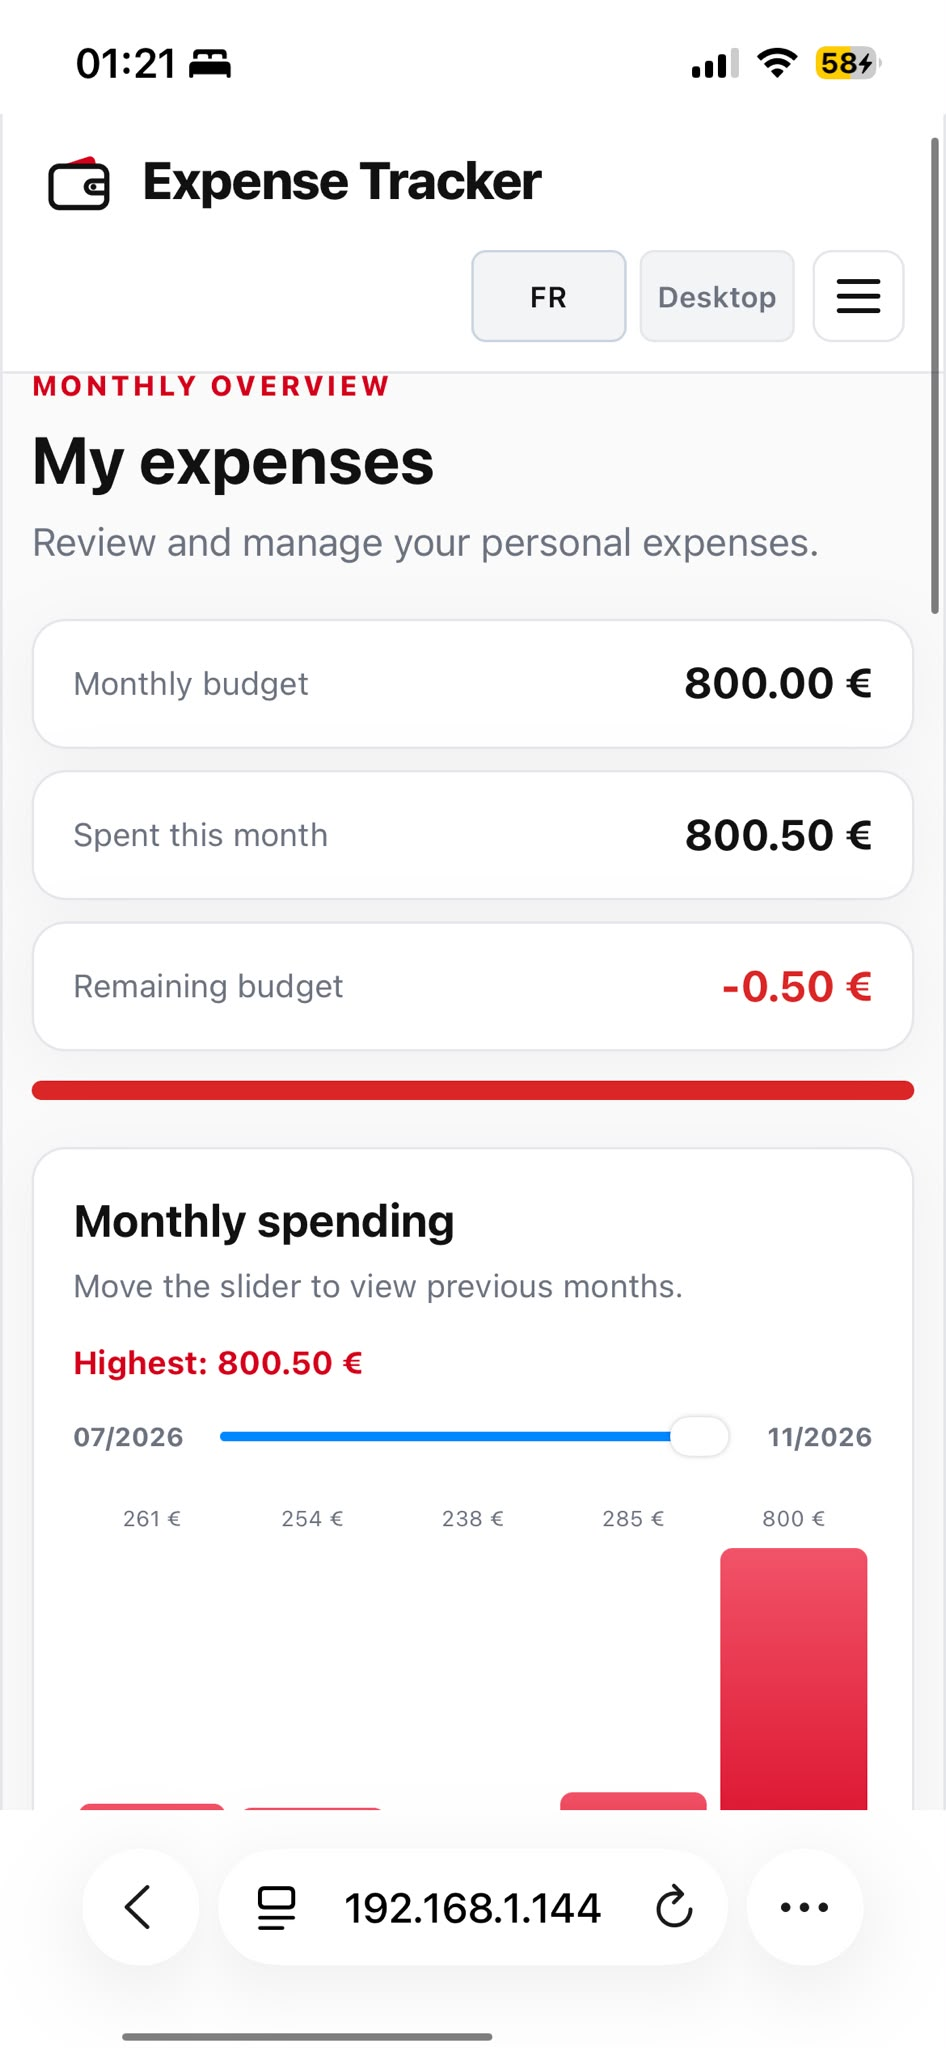
\includegraphics[width=.49\linewidth,height=.29\textheight,keepaspectratio]{my_expense_en_m.jpeg}
\end{center}

\subsection*{Contact}
\begin{center}
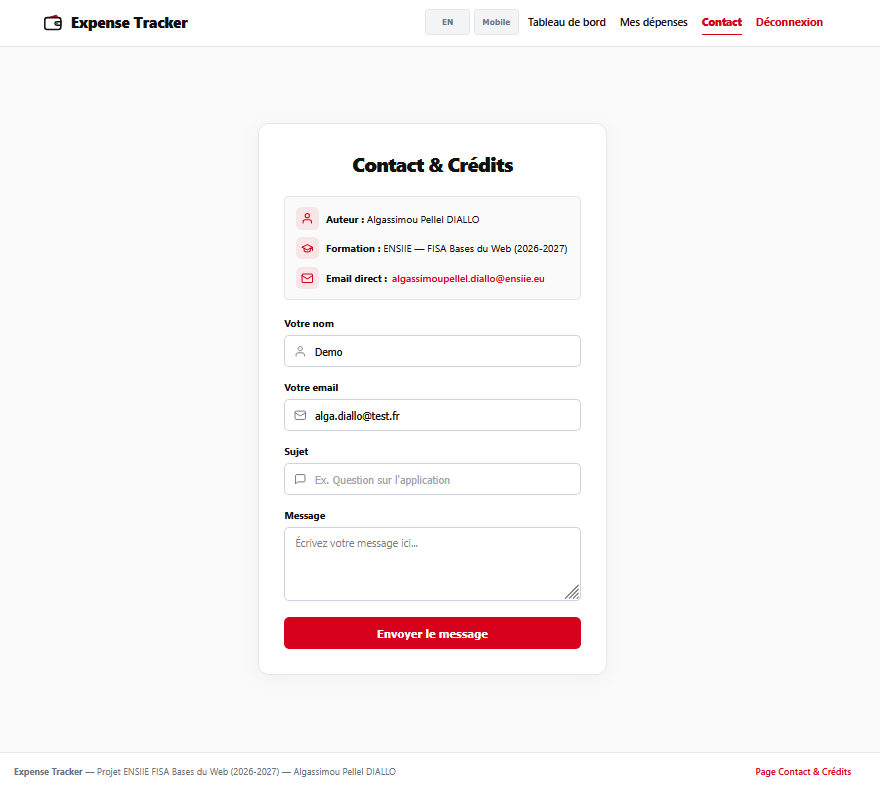
\includegraphics[width=.49\linewidth,height=.29\textheight,keepaspectratio]{contact_fr_laptop.png}
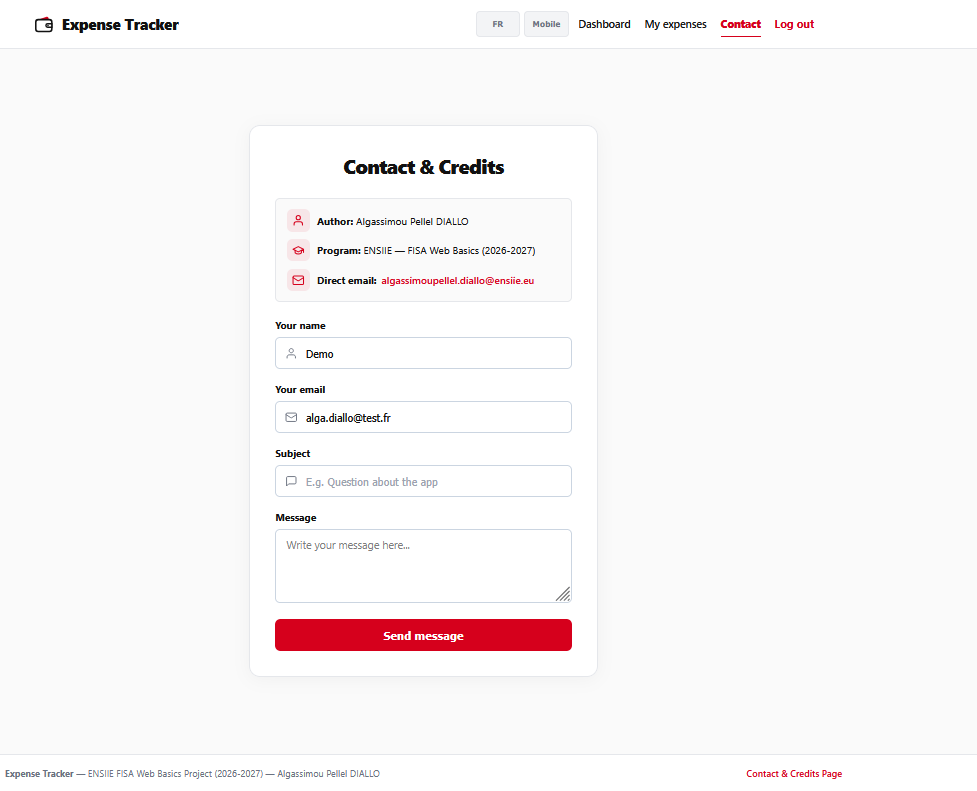
\includegraphics[width=.49\linewidth,height=.29\textheight,keepaspectratio]{contact_en_laptop.png}\\
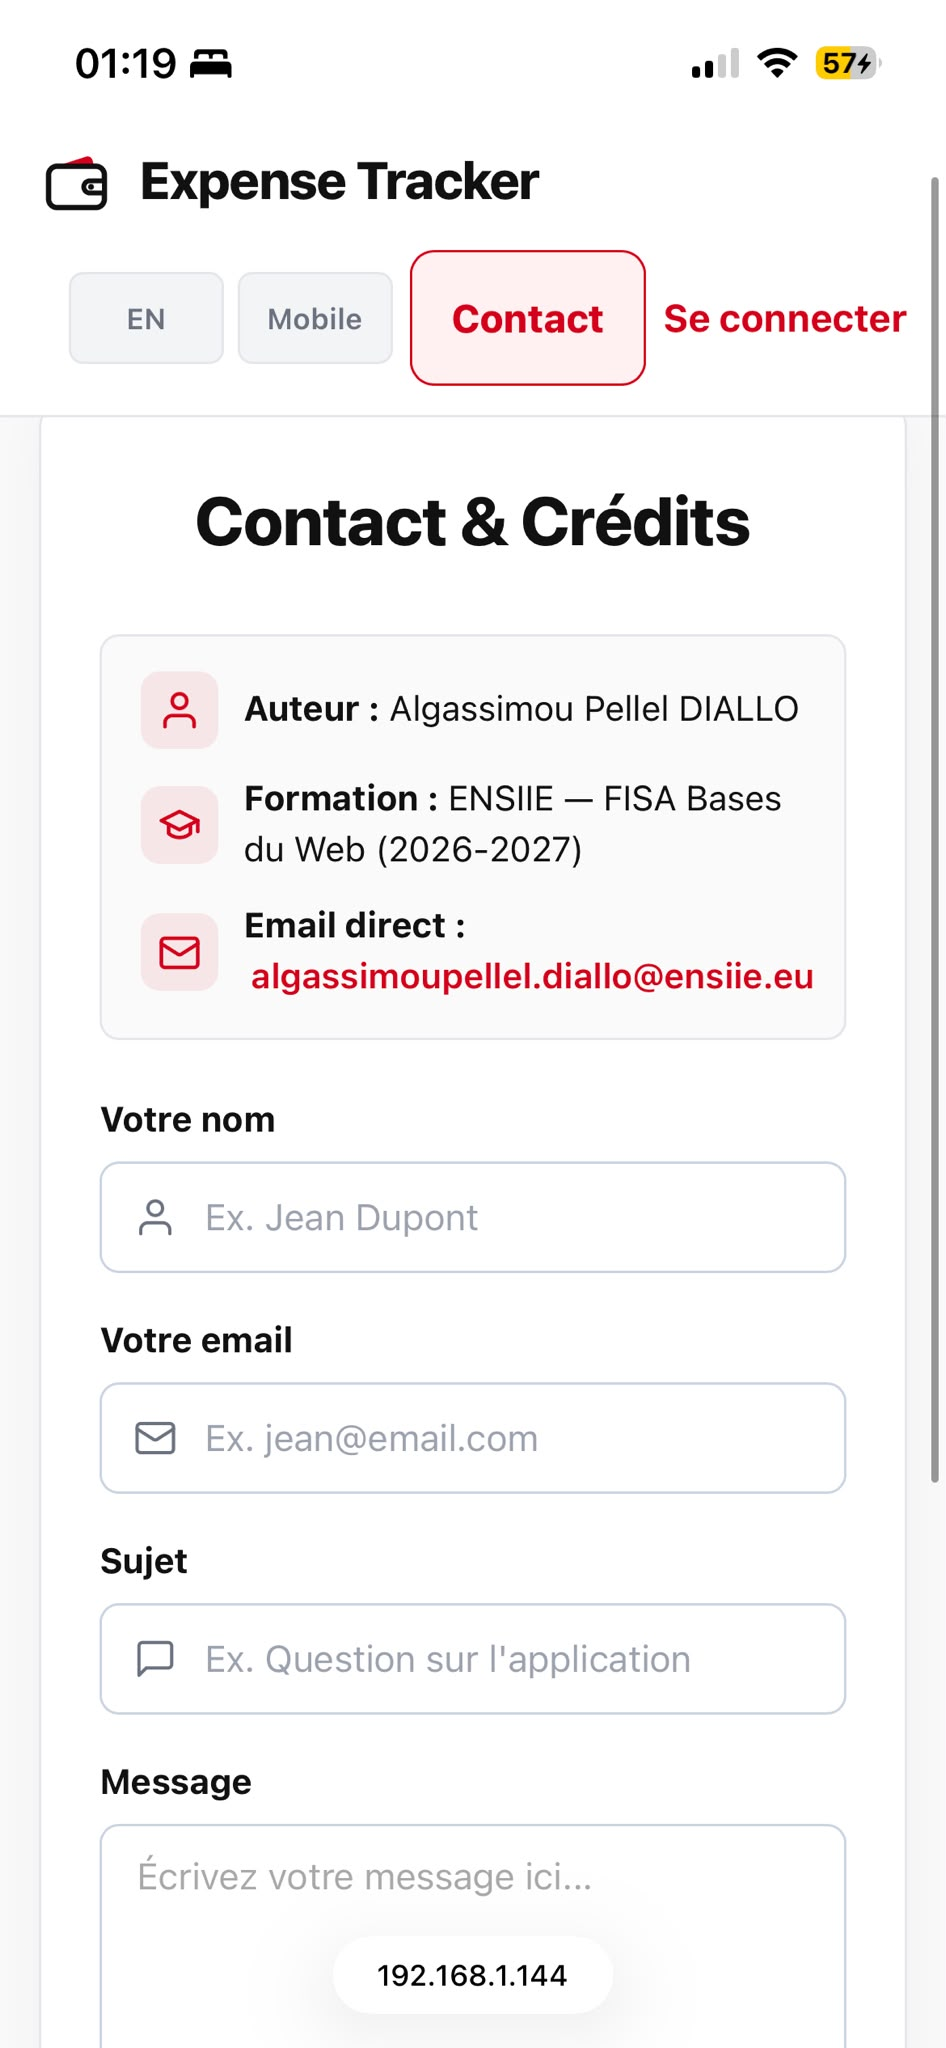
\includegraphics[width=.49\linewidth,height=.29\textheight,keepaspectratio]{contact_Fr_m.jpeg}
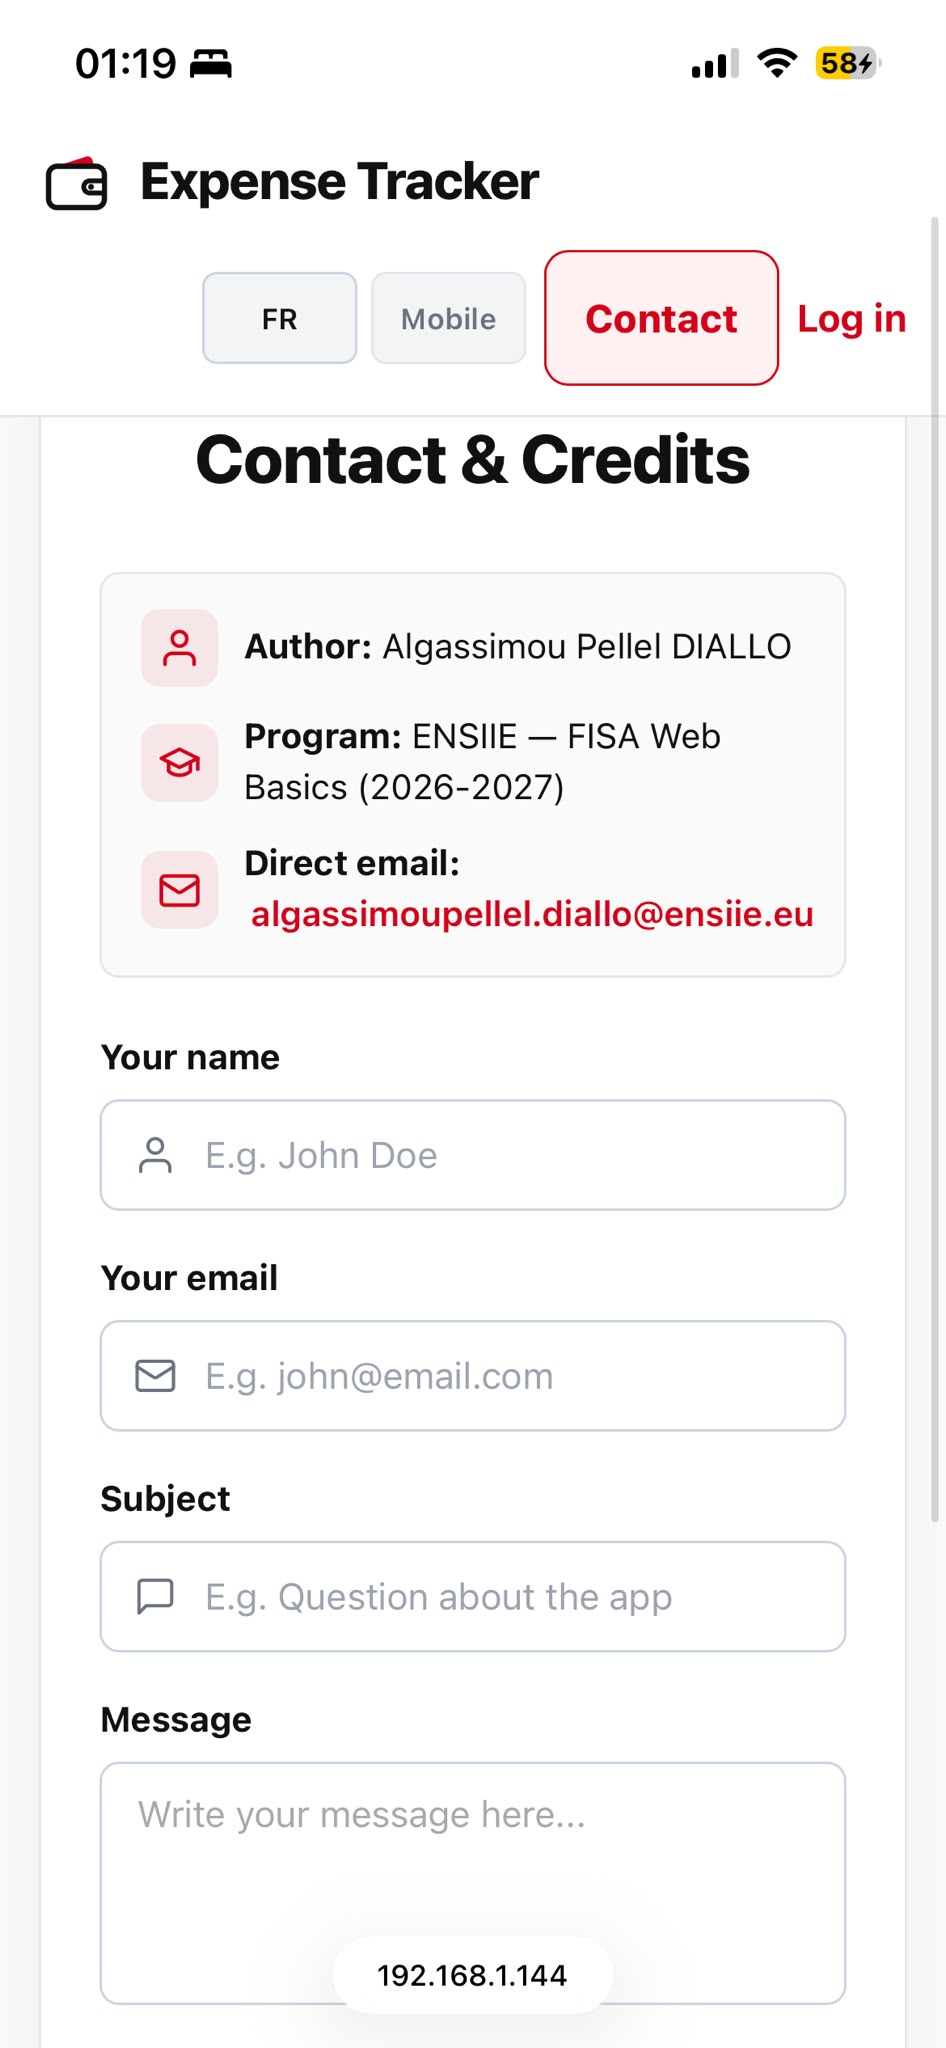
\includegraphics[width=.49\linewidth,height=.29\textheight,keepaspectratio]{contact_en_m.jpeg}
\end{center}

\end{document}
